\appendix

\section{Archivos de diferencias}\label{appendix:apA}

\subsection{\textit{sched\_switch} (v12 a v13): Firma de la función y variables}\label{appendix:apA1}

\begin{lstlisting}[language=diff]
- void sched_switch(struct thread *td, struct thread *newtd, int flags)
+ void sched_switch(struct thread *td, int flags)
{
+   struct thread *newtd;
    struct mtx *tmtx;
    struct td_sched *ts;
    struct proc *p;
    int preempted;

-   tmtx = NULL;
+   tmtx = &sched_lock;
    ts = td_get_sched(td);
    p = td->td_proc;

    THREAD_LOCK_ASSERT(td, MA_OWNED);
...
}
\end{lstlisting}



\subsection{\textit{sched\_switch} (v12 a v13): Cambio de posición del bloque que bloquea el hilo previo al \textit{resource\_expulse\_thread}}\label{appendix:apA2}

\begin{lstlisting}[language=diff]
+   if (td->td_lock != &sched_lock) {
+   	mtx_lock_spin(&sched_lock);
+   	tmtx = thread_lock_block(td);
+   	mtx_unlock_spin(tmtx);
+   }

   if ((td->td_flags & TDF_NOLOAD) == 0)
   	sched_load_rem();

    td->td_lastcpu = td->td_oncpu;
    preempted = (td->td_flags & TDF_SLICEEND) == 0 && (flags & SW_PREEMPT) != 0;
    td->td_flags &= ~(TDF_NEEDRESCHED | TDF_SLICEEND);
    td->td_owepreempt = 0;
    td->td_oncpu = NOCPU;

    resource_expulse_thread(td, flags);

-   if (td->td_lock != &sched_lock) {
-   	mtx_lock_spin(&sched_lock);
-   	tmtx = thread_lock_block(td);
-   	mtx_unlock_spin(tmtx);
-   }
...
\end{lstlisting}


\subsection{\textit{sched\_switch} (v12 a v13): Selección y ejecución de un nuevo thread}\label{appendix:apA3}

\begin{lstlisting}[language=diff]
+   newtd = choosethread();
-   if (newtd) {
-       /*
-        * The thread we are about to run needs to be counted
-        * as if it had been added to the run queue and selected.
-        * It came from:
-        * * A preemption
-        * * An upcall
-        * * A followon
-        */
-       KASSERT((newtd->td_inhibitors == 0),
-           ("trying to run inhibited thread"));
-       newtd->td_flags |= TDF_DIDRUN;
-           TD_SET_RUNNING(newtd);
-       if ((newtd->td_flags & TDF_NOLOAD) == 0)
-           sched_load_add();
-       if (ts->ts_runq != &runq){
-           resource_fire_net(newtd, TRAN_UNQUEUE + (PCPU_GET(cpuid)*CPU_BASE_TRANSITIONS));
-       }
-       else{
-           resource_fire_net(newtd, TRAN_FROM_GLOBAL_CPU + (PCPU_GET(cpuid)*CPU_BASE_TRANSITIONS));
-       }
-   } else {
-       newtd = choosethread();
-       MPASS(newtd->td_lock == &sched_lock);
-   }

    resource_execute_thread(newtd, PCPU_GET(cpuid));

\end{lstlisting}

\section{Detalles de la implementación del módulo de monopolizado}\label{appendix:apB}

En este apartado se desarrollará con mayor profundidad la implementación del módulo de monopolización de hilos, haciendo referencia principalmente a las funciones que se han modificado y su comportamiento a lo largo del proceso de ejecución de un hilo.

El planificador 4BSD maneja los cambios de contexto cuando un hilo termina su ejecución o queda bloqueado, generando una interrupción para seleccionar un nuevo hilo.

La función principal para gestionar estos cambios es \textit{mi\_switch()}, que invoca a \textit{sched\_switch()}. Esta función se encarga de preparar el nuevo hilo para su ejecución y usa \textit{sched\_add()} para añadirlo a la cola de un procesador, considerando la afinidad y las políticas del planificador. Luego, \textit{sched\_choose()} selecciona el hilo a ejecutar y realiza el cambio de contexto en caso de ser necesario.

Para integrar el módulo de monopolización, modificamos \textit{sched\_add()} para permitir que ciertos hilos se fijen a CPUs específicas. Esto asegura que un CPU ejecute siempre el mismo hilo hasta que se decida lo contrario, excluyendo así, a todos aquellos hilos con un identificador diferente al elegido.

Comenzamos implementando un arreglo llamado \textit{pinned\_threads\_per\_cpu}, que almacena el identificador (ID) del hilo asignado a cada CPU. El arreglo contiene tantos elementos como CPU's existan en el sistema, es decir, para un procesador de cuatro núcleos, el arreglo contendrá cuatro elementos. Cada elemento será el encargado de guardar el valor del identificador del hilo que monopoliza la CPU correspondiente.  Si un CPU está libre, el valor en el arreglo es -1.

En el siguiente ejemplo, se detalla un caso en el que el hilo con ID 100101 tomó control sobre la CPU1 y donde el resto de los procesadores se encuentran funcionando normalmente.

int \textit{pinned\_threads\_per\_cpu}[CPU\_NUMBER] = \{ -1, 100101, -1, -1 \};

Al momento de encolar el hilo, se busca cuál de los procesadores disponibles sería la mejor opción para continuar la ejecución del mismo. Ésta decisión se toma dentro del método \textit{resource\_choose\_cpu} desarrollado en el trabajo integrador previo y extendido actualmente, para hacer uso de este nuevo arreglo de hilos asociados a procesadores. El método recibe como parámetro el hilo que se quiera encolar, y realiza tres operaciones condicionales que determinarán el procesador a elegir:

\begin{itemize}
    \item Como primera condición, si el hilo se encuentra dentro del arreglo de \textit{pinned\_threads\_per\_cpu} ya estamos en condiciones de elegir dicho procesador como el indicado para el encolado.
    \item Si el hilo no se encuentra dentro del arreglo, se intenta asignar a la cola del último procesador en el que se ejecutó. Esto es posible solo si la transición TRAN\_ADDTOQUEUE de dicho procesador se encuentra sensibilizada y el procesador no está monopolizado por otro hilo.
    \item Por último, si no se cumplen ninguna de las dos condiciones previas, se recorren los diferentes núcleos del procesador y se retorna el primero que cumpla las condiciones necesarias para el encolado.
\end{itemize}

Como parte del desarrollo del módulo, también se implementaron algunos métodos complementarios encargados de manejar el estado del arreglo \textit{pinned\_threads\_per\_cpu}.

\begin{itemize}
    \item \textit{toggle\_pin\_thread\_to\_cpu()}: Método encargado de conmutar el estado de monopolización de un procesador. Recibe el ID de un hilo y de un procesador como parámetros y realiza diferentes operaciones de acuerdo al estado del arreglo:
          \begin{itemize}
              \item Si el procesador se encuentra libre, se agrega el ID del hilo a la posición correspondiente en el arreglo.
              \item Si el procesador ya estaba monopolizado por otro hilo, se sobrescribe con el nuevo ID.
              \item En caso de que el hilo ya se encuentre monopolizando al procesador, lo libera escribiendo el valor -1 en la posición correspondiente.
          \end{itemize}
    \item \textit{cpu\_available\_for\_thread()}: Método utilizado por \textit{resource\_choose\_cpu} para saber si un hilo puede utilizar un procesador, o si este se encuentra monopolizado por otro. Recibe el ID de un hilo y de un procesador como parámetros y retorna 1 en caso de que el procesador se encuentre habilitado para encolar dicho hilo; retorna 0 en caso de que dicho procesador se encuentre tomado por otro hilo.
    \item \textit{get\_monopolized\_cpu\_by\_thread\_id()}: Método utilizado por \textit{resource\_choose\_cpu} para obtener el ID del procesador al que se encuentra asociado el hilo enviado por parámetro. Retorna -1 en caso de que no esté anclado a ningún CPU.\par
\end{itemize}

\section{Análisis de \textit{kernel panic} debido a fallos de página (\textit{page fault})}\label{appendix:apC}

Se analizaron archivos \textit{dump} generados en un sistema FreeBSD a partir de un page fault ocurrido mientras la placa de red se encontraba encendida. El proceso involucrado en el fallo es sshd, que generó un \textit{kernel panic} debido a un acceso inválido a memoria.

El proceso de análisis inició cargando el archivo de \textit{core dump} con la herramienta \textit{kgdb}, que permite depurar el \textit{kernel} de FreeBSD y obtener información detallada sobre el estado del sistema al momento del fallo.

Todos los archivos de \textit{core dump} generados por el sistema se encuentran en la carpeta \textit{/var/crash/}, y para cargarlos en \textit{kgdb} se utiliza el comando \textit{kgdb /boot/kernel/kernel /var/crash/vmcore.0}.

En las imagenes a continuación se muestran algunas de las salidas obtenidas durante el análisis del \textit{core dump}. Una vez cargado el \textit{core dump}, se utilizó el comando \textit{where} para obtener la ubicación del fallo de página en el \textit{kernel}. La salida de este comando muestra la pila de llamadas al momento del fallo, y se observa que el fallo ocurrió en la función \textit{kern\_select}.

Para obtener más información sobre el fallo, se utilizó el comando \textit{up} para navegar hacia la función \textit{kern\_select}.

\begin{figure}[H]
    \centering
    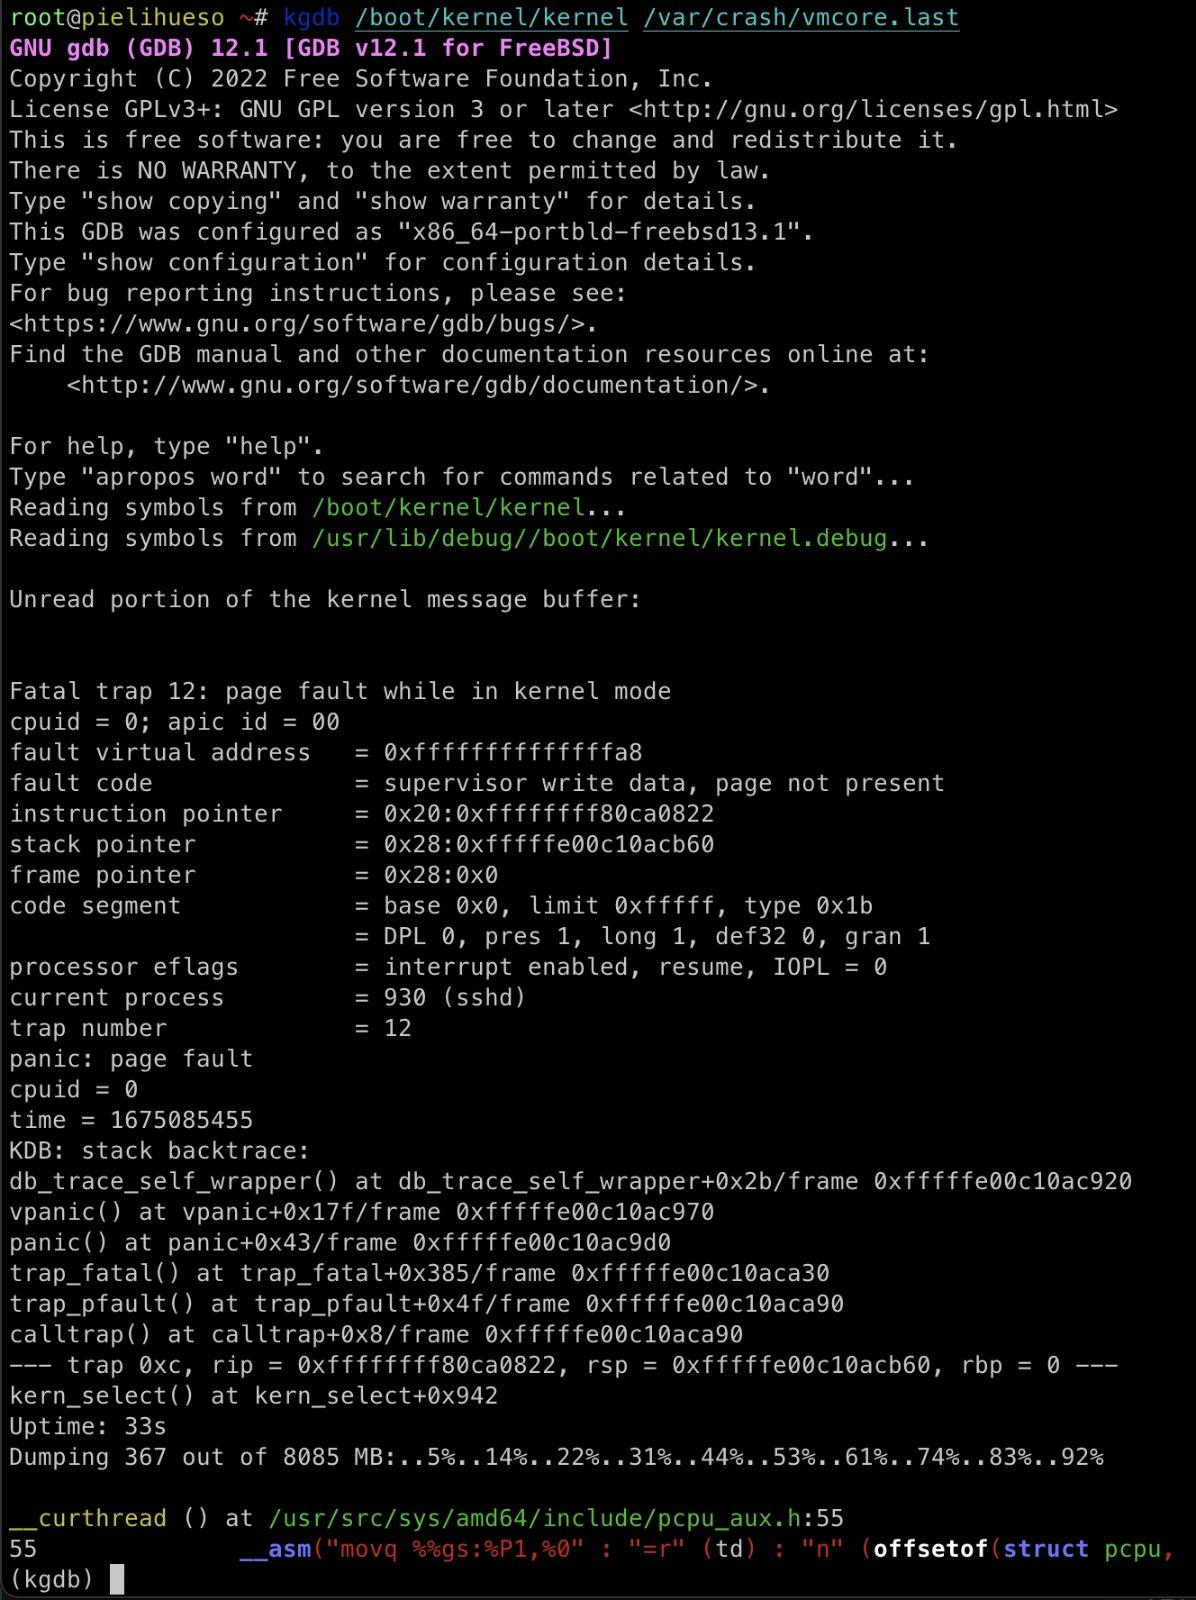
\includegraphics[width=0.8\textwidth]{images/kgdb_init.jpeg}
    \caption{Inicialización de \textit{kgdb} y lectura del \textit{crash dump}.}
    \label{fig:kgdb_init}
\end{figure}

\vspace{.50cm}
\begin{figure}[H]
    \centering
    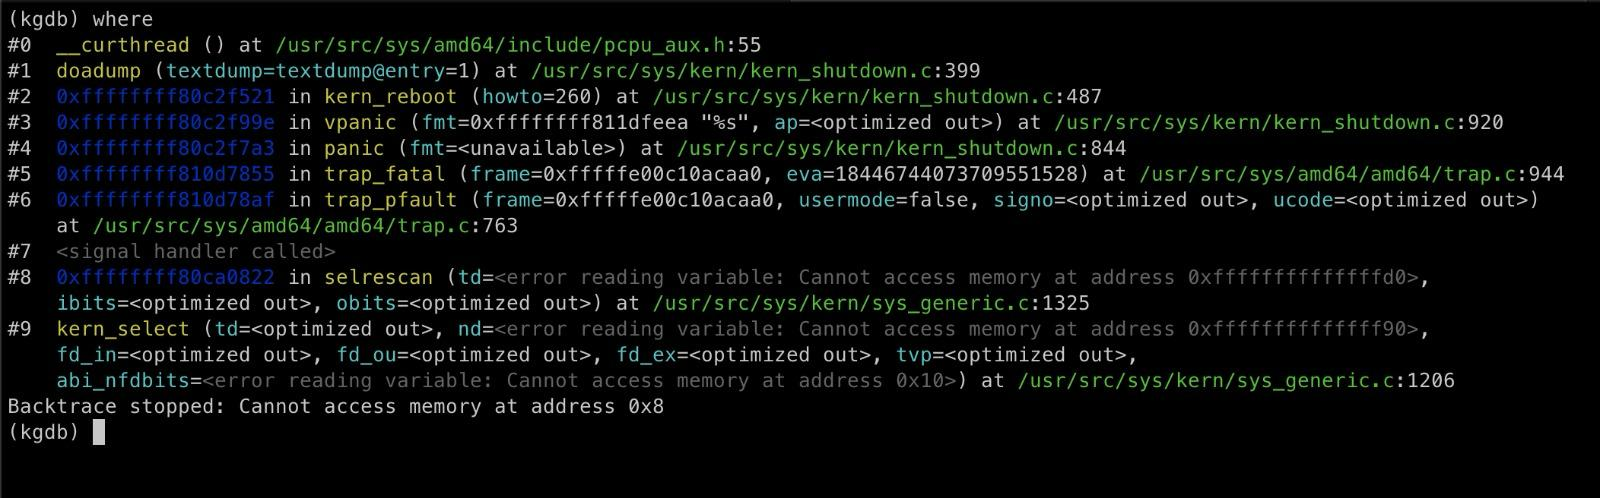
\includegraphics[width=1\textwidth]{images/kgdb_where.jpeg}
    \caption{Ubicación del fallo de página en el \textit{kernel}.}
    \label{fig:kgdb_where}
\end{figure}

\vspace{.50cm}
\begin{figure}[H]
    \centering
    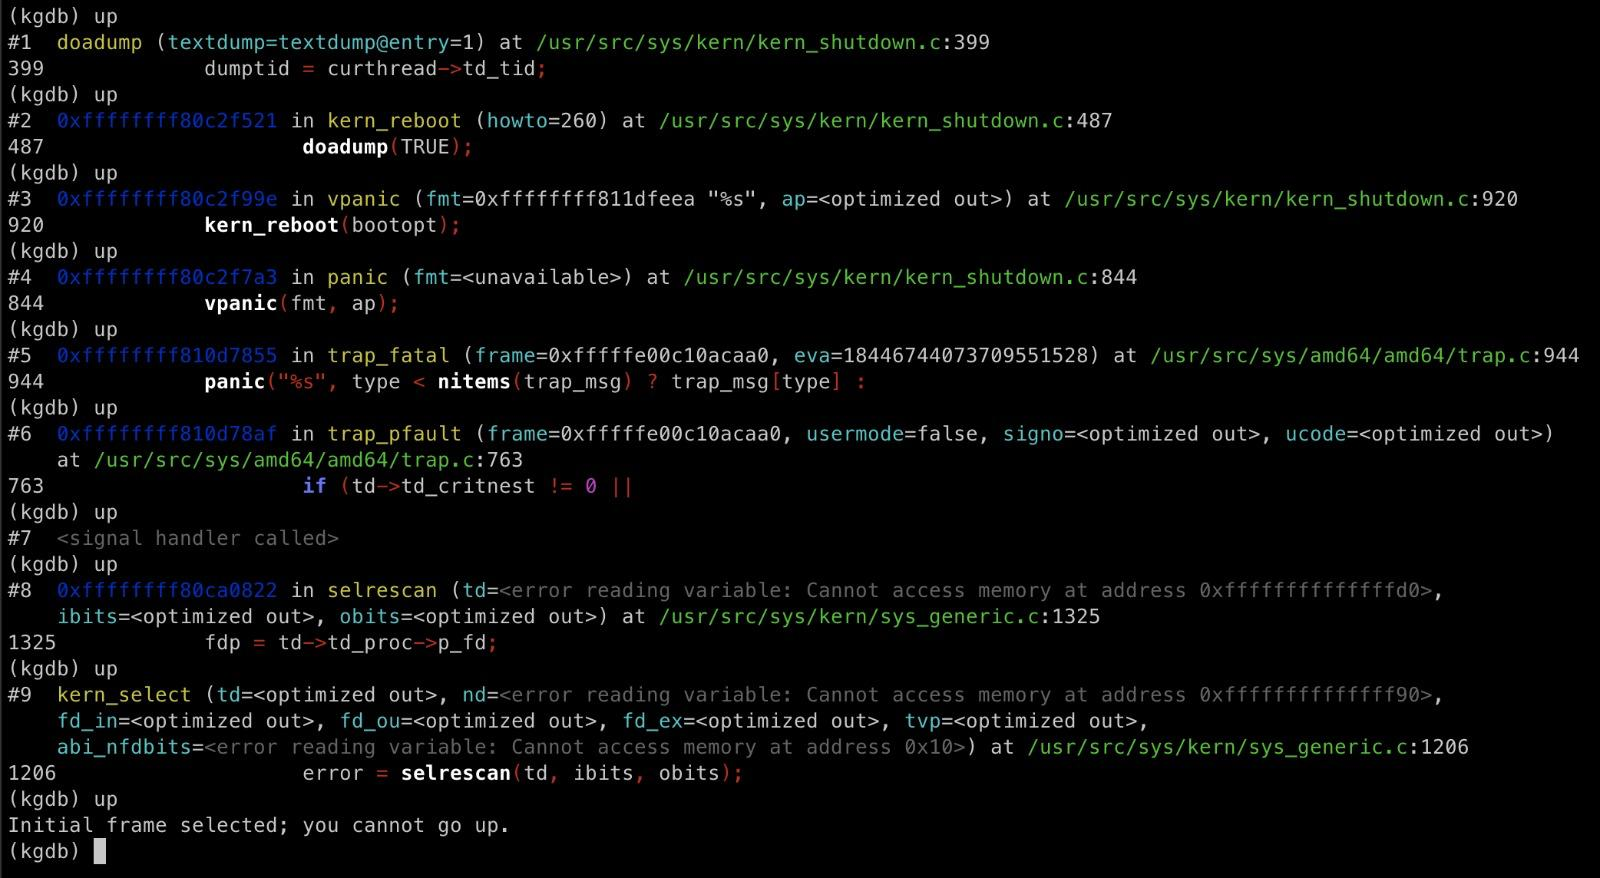
\includegraphics[width=1\textwidth]{images/kgdb_kern-select.jpeg}
    \caption{Llamada a la función \textit{kern\_select} en el \textit{kernel}.}
    \label{fig:kgdb_kern-select}
\end{figure}

\section{Ejecución del programa de estrés con diferentes cantidades de núcleos activos}\label{appendix:apD}

\begin{figure}[H]
    \centering
    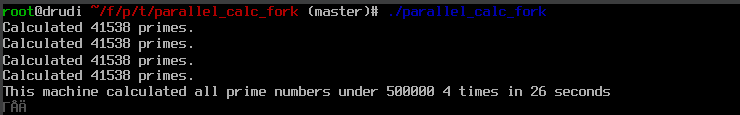
\includegraphics[width=1\textwidth]{images/cpuOnOff-4CPUsTime.png}
    \caption{Tiempo de ejecución del programa de estrés con 4 núcleos activos.}
    \label{fig:cpuOnOff-4CPUsTime}
\end{figure}

\begin{figure}[H]
    \centering
    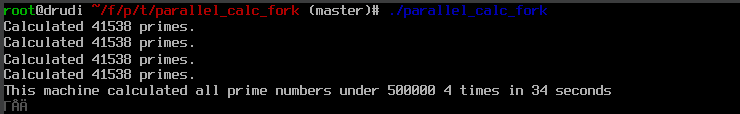
\includegraphics[width=1\textwidth]{images/cpuOnOff-3CPUsTime.png}
    \caption{Tiempo de ejecución del programa de estrés con 3 núcleos activos.}
    \label{fig:cpuOnOff-3CPUsTime}
\end{figure}

\begin{figure}[H]
    \centering
    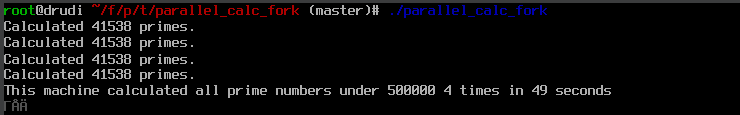
\includegraphics[width=1\textwidth]{images/cpuOnOff-2CPUsTime.png}
    \caption{Tiempo de ejecución del programa de estrés con 2 núcleos activos.}
    \label{fig:cpuOnOff-2CPUsTime}
\end{figure}


% Add more sections as needed before the \end{document} command.
\end{document}
